% Copyright 2006 by Till Tantau
%
% This file may be distributed and/or modified
%
% 1. under the LaTeX Project Public License and/or
% 2. under the GNU Free Documentation License.
%
% See the file doc/generic/pgf/licenses/LICENSE for more details.


\section{Mindmap Drawing Library}

\begin{tikzlibrary}{mindmap}
    This packages provides styles for drawing mindmap diagrams.
\end{tikzlibrary}
%
\begin{codeexample}[setup code,hidden]
    \usetikzlibrary{mindmap}
\end{codeexample}


\subsection{Overview}

This library is intended to make the creation of mindmaps or concept maps
easier. A \emph{mindmap} is a graphical representation of a concept together
with related concepts and annotations. Mindmaps are, essentially, trees,
possibly with a few extra edges added, but they are usually drawn in a special
way: The root concept is placed in the middle of the page and is drawn as a
huge circle, ellipse, or cloud. The related concepts then ``leave'' this root
concept via branch-like tendrils.

The mindmap library of \tikzname\ produces mindmaps that look a bit different
from the standard mindmaps: While the big root concept is still a circle,
related concepts are also depicted as (smaller) circles. The related concepts
are linked to the root concept via organic-looking connections. The overall
effect is visually rather pleasing, but readers may not immediately think of a
mindmap when they see a picture created with this library.

Although it is not strictly necessary, you will usually create mindmaps using
\tikzname's tree mechanism and some of the styles and macros of the package
work best when used inside trees. However, it is still possible and sometimes
necessary to treat parts of a mindmap as a graph with arbitrary edges and this
is also possible.


\subsection{The Mindmap Style}

Every mindmap should be put in a scope or a picture where the |mindmap| style
is used. This style installs some internal settings.

\begin{stylekey}{/tikz/mindmap}
    Use this style with all pictures or at least scopes that contain a mindmap.
    It installs a whole bunch of settings that are useful for drawing mindmaps.
    %
\begin{codeexample}[]
\tikz[mindmap,concept color=red!50]
  \node [concept] {Root concept}
    child[grow=right] {node[concept] {Child concept}};
\end{codeexample}
    %
    The sizes of concepts are predefined in such a way that a medium-size
    mindmap will fit on an A4 page (more or less).
    %
    \begin{stylekey}{/tikz/every mindmap}
        This style is included by the |mindmap| style. Change this style to add
        special settings to your mindmaps.
        %
\begin{codeexample}[]
\tikz[large mindmap,concept color=red!50]
  \node [concept] {Root concept}
    child[grow=right] {node[concept] {Child concept}};
\end{codeexample}
    \end{stylekey}

    \paragraph{Remark:}
    Note that |mindmap| redefines |font| sizes and |sibling angle| depending on
    the current concept level (i.e. inside of |level 1 concept|,
    |level 2 concept| etc.). Thus, if you need to redefine these variables, use

    |level 1 concept/.append style={font=\small}|

    \noindent or

    |level 2 concept/.append style={sibling distance=90}|

    \noindent \emph{after} the |mindmap| style.
\end{stylekey}

\begin{stylekey}{/tikz/small mindmap}
    This style includes the |mindmap| style, but additionally changes the
    default size of concepts, fonts and distances so that a medium-sized
    mindmap will fit on an A5 page (A5 pages are half as large as A4 pages).
    Mindmaps with |small mindmap| will also fit onto a standard frame of the
    |beamer| package.
\end{stylekey}

\begin{stylekey}{/tikz/large mindmap}
    This style includes the |mindmap| style, but additionally changes the
    default size of concepts, fonts and distances so that a medium-sized
    mindmap will fit on an A3 page (A3 pages are twice as large as A4 pages).
\end{stylekey}

\begin{stylekey}{/tikz/huge mindmap}
    This style causes concepts to be even bigger and it is best used with A2
    paper and above.
\end{stylekey}


\subsection{Concepts Nodes}

The basic entities of mindmaps are called \emph{concepts} in \tikzname. A
concept is a node of style |concept| and it must be circular for some of the
connection macros to work.


\subsubsection{Isolated Concepts}

The following styles influence how isolated concepts are rendered:

\begin{stylekey}{/tikz/concept}
    This style should be used with all nodes that are concepts, although some
    styles like |extra concept| install this style automatically.

    Basically, this style makes the concept node circular and installs a
    uniform color called |concept color|, see below. Additionally, the style
    |every concept| is called.
    %
\begin{codeexample}[]
\tikz[mindmap,concept color=red!50] \node [concept] {Some concept};
\end{codeexample}

    \begin{stylekey}{/tikz/every concept}
        In order to change the appearance of concept nodes, you should change
        this style. Note, however, that the color of a concept should be
        uniform for some of the connection bar stuff to work, so you should not
        change the color or the draw/fill state of concepts using this option.
        It is mostly useful for changing the text color and font.
    \end{stylekey}

    \begin{key}{/tikz/concept color=\meta{color}}
        This option tells \tikzname\ which color should be used for filling and
        stroking concepts. The difference between this option and just setting
        |every concept| to the desired color is that this option allows
        \tikzname\ to keep track of the colors used for concepts. This is
        important when you \emph{change} the color between two connected
        concepts. In this case, \tikzname\ can automatically create a shading
        that provides a smooth transition between the old and the new concept
        color; we will come back to this in the next section.
    \end{key}
\end{stylekey}

\begin{stylekey}{/tikz/extra concept}
    This style is intended for concepts that are not part of the ``mindmap
    tree'', but stand beside it. Typically, they will have a subdued color or
    be smaller. In order to have these concepts appear in a uniform way and in
    order to indicate in the code that these concepts are additional, you can
    use this style.
    %
\begin{codeexample}[]
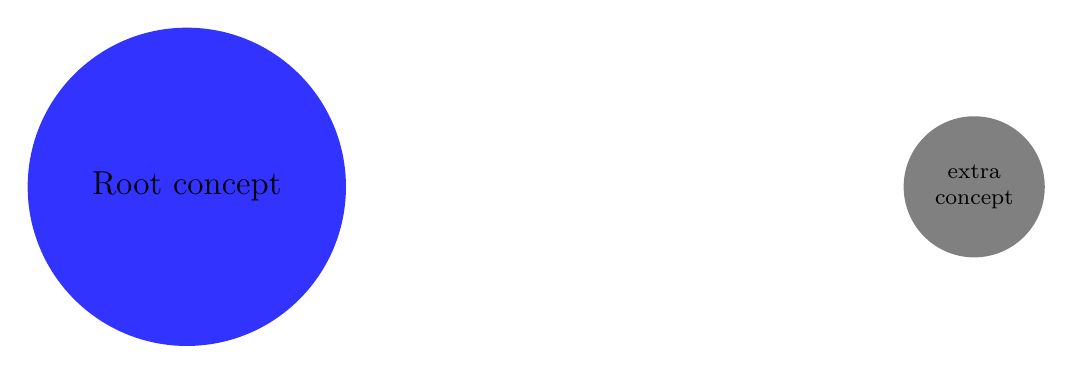
\begin{tikzpicture}[mindmap,concept color=blue!80]
  \node [concept]                 {Root concept};
  \node [extra concept] at (10,0) {extra concept};
\end{tikzpicture}
\end{codeexample}
    %
    \begin{stylekey}{/tikz/every extra concept}
        Change this style to change the appearance of extra concepts.
    \end{stylekey}
\end{stylekey}


\subsubsection{Concepts in Trees}

As pointed out earlier, \tikzname\ assumes that your mindmap is built using the
|child| facilities of \tikzname. There are numerous options that influence how
concepts are rendered at the different levels of a tree.

\begin{stylekey}{/tikz/root concept}
    This style is used for the roots of mindmap trees. By adding something to
    this, you can change how the root of a mindmap will be rendered.
    %
\begin{codeexample}[]
\tikz
  [root concept/.append style={concept color=blue!80,minimum size=3.5cm},
   mindmap]
  \node [concept] {Root concept};
\end{codeexample}

    Note that styles like |large mindmap| redefine these styles, so you should
    add something to this style only inside the picture.
\end{stylekey}

\begin{stylekey}{/tikz/level 1 concept}
    The |mindmap| style adds this style to the |level 1| style. This means that
    the first level children of a mindmap tree will use this style.
    %
\begin{codeexample}[]
\tikz
  [root concept/.append style={concept color=blue!80},
   level 1 concept/.append style={concept color=red!50},
   mindmap]
  \node [concept] {Root concept}
    child[grow=30] {node[concept] {child}}
    child[grow=0 ] {node[concept] {child}};
\end{codeexample}
\end{stylekey}

\begin{stylekey}{/tikz/level 2 concept}
    Works like |level 1 concept|, only for second level children.
\end{stylekey}

\begin{stylekey}{/tikz/level 3 concept}
    Works like |level 1 concept|.
\end{stylekey}

\begin{stylekey}{/tikz/level 4 concept}
    Works like |level 1 concept|. Note that there are no fifth and higher level
    styles, you need to modify |level 5| directly in such cases.
\end{stylekey}

\begin{key}{/tikz/concept color=\meta{color}}
    We saw already that this option is used to change the color of concepts. We
    now have a look at its effect when used on child nodes of a concept.
    Normally, this option simply changes the color of the children. However,
    when the option is given as an option to the |child| operation (and not to
    the |node| operation and also not as an option to all children via the
    |level 1| style), \tikzname\ will smoothly change the concept color from
    the parent's color to the color of the child concept.

    Here is an example:
    %
\begin{codeexample}[]
\tikz[mindmap,concept color=blue!80]
  \node [concept] {Root concept}
    child[concept color=red,grow=30] {node[concept] {Child concept}}
    child[concept color=orange,grow=0]  {node[concept] {Child concept}};
\end{codeexample}

    In order to have a concept color which changes with the hierarchy level, a
    tiny bit of magic is needed:
% FIXME: is this a bug in the software!? The root concept is black!?
\begin{codeexample}[]
\tikz[mindmap,text=white,
      root concept/.style={concept color=blue},
      level 1 concept/.append style=
        {every child/.style={concept color=blue!50}}]
  \node [concept] {Root concept}
    child[grow=30] {node[concept] {child}}
    child[grow=0 ] {node[concept] {child}};
\end{codeexample}
    %
\end{key}


\subsection{Connecting Concepts}

\subsubsection{Simple Connections}

The easiest way to connect two concepts is to draw a line between them. In
order to give such lines a consistent appearance, it is recommendable to use
the following style when drawing such lines:

\begin{stylekey}{/tikz/concept connection}
    This style can be used for lines between two concepts. Feel free to
    redefine this style.
\end{stylekey}

A problem arises when you need to connect concepts after the main mindmap has
been drawn. In this case you will want the connection lines to lie
\emph{behind} the main mindmap. However, you can draw the lines only after the
coordinates of the concepts have been determined. In this case you should place
the connecting lines on a background layer as in the following example:

\begin{codeexample}[preamble={\usetikzlibrary{backgrounds}}]
\begin{tikzpicture}
  [root concept/.append style={concept color=blue!20,minimum size=2cm},
   level 1 concept/.append style={sibling angle=45},
   mindmap]
  \node [concept] {Root concept}
    [clockwise from=45]
    child { node[concept] (c1) {child}}
    child { node[concept] (c2) {child}}
    child { node[concept] (c3) {child}};
  \begin{pgfonlayer}{background}
    \draw [concept connection]  (c1) edge (c2)
                                     edge (c3)
                                (c2) edge (c3);
  \end{pgfonlayer}
\end{tikzpicture}
\end{codeexample}


\subsubsection{The Circle Connection Bar Decoration}

Instead of a simple line between two concepts, you can also add a bar between
the two nodes that has slightly organic ends. These bars are also used by
default as the edges from parents in the mindmap tree.

For the drawing of the bars a special decoration is used, which is defined in
the mindmap library:

\begin{decoration}{circle connection bar}
    This decoration can be used to connect two circles. The start of the
    to-be-decorated path should lie on the border of the first circle, the end
    should lie on the border of the second circle. The following two decoration
    keys should be initialized with the sizes of the circles:
    %
    \begin{itemize}
        \item |start radius|
        \item |end radius|
    \end{itemize}
    %
    Furthermore, the following two decoration keys influence the decoration:
    %
    \begin{itemize}
        \item |amplitude|
        \item |angle|
    \end{itemize}
    %
    The decoration turns a straight line into a path that starts on the border
    of the first circle at the specified angle relative to the line connecting
    the centers of the circles. The path then changes into a rectangle whose
    thickness is given by the amplitude. Finally, the path ends with the same
    angles on the second circle.

    Here is an example that should make this clearer:
    %
\begin{codeexample}[]
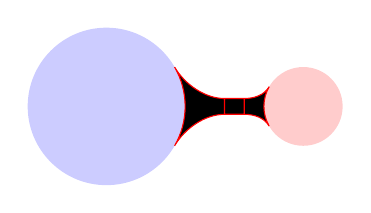
\begin{tikzpicture}
    [decoration={start radius=1cm,end radius=.5cm,amplitude=2mm,angle=30}]
  \fill[blue!20] (0,0)   circle (1cm);
  \fill[red!20]  (2.5,0) circle (.5cm);

  \filldraw [draw=red,fill=black,
             decorate,decoration=circle connection bar] (1,0) -- (2,0);
\end{tikzpicture}
\end{codeexample}

    As can be seen, the decorated path consists of three parts and is not
    really useful for drawing. However, if you fill the decorated path only,
    and if you use the same color as for the circles, the result is better.
    %
\begin{codeexample}[]
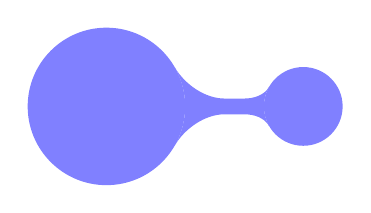
\begin{tikzpicture}
  [blue!50,decoration={start radius=1cm,
                       end radius=.5cm,amplitude=2mm,angle=30}]
  \fill (0,0)   circle (1cm);
  \fill (2.5,0) circle (.5cm);

  \fill [decorate,decoration=circle connection bar] (1,0) -- (2,0);
\end{tikzpicture}
\end{codeexample}

    In the above example you may notice the small white line between the
    circles and the decorated path. This is due to rounding errors.
    Unfortunately, for larger distances, the errors can accumulate quite
    strongly, especially since \tikzname\ and \TeX\ are not very good at
    computing square roots. For this reason, it is a good idea to make the
    circles slightly larger to cover up such problems. When using nodes of
    shape |circle|, you can just add the |draw| option with a |line width| of
    one or two points (for very large distances you may need line width up to
    4pt).
    %
\begin{codeexample}[]
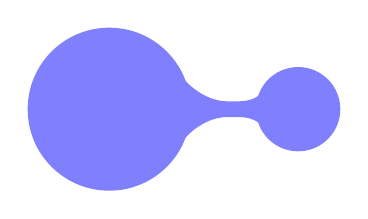
\begin{tikzpicture}
  [blue!50,decoration={start radius=1cm,
                       end radius=.5cm,amplitude=2mm,angle=30}]
  \fill (0,0)   circle (1cm+1pt);
  \fill (2.4,0) circle (.5cm+1pt);

  \fill [decorate,decoration=circle connection bar] (1,0) -- (1.9,0);
\end{tikzpicture}
\end{codeexample}

    % FIXME: this paragraph appears to be deprecated:
    %Note the slightly strange |outer sep=0pt|. This is needed so that
    %the decorated path lies on the border of the filled circle, not on the
    %border of the stroked circle (which is slightly larger and this
    %slightly larger size is exactly what we wish to use to cover up the
    %rounding errors).
\end{decoration}


\subsubsection{The Circle Connection Bar To-Path}

The |circle connection bar| decoration is a bit complicated to use. Especially
specifying the radii is quite bothersome (the amplitude and the angle can be
set once and for all). For this reason, the mindmap library defines a special
to-path that performs the necessary computations for you.

\begin{stylekey}{/tikz/circle connection bar}
    This style installs a rather involved to-path. Unlike normal to-paths, this
    path requires that the start and the target of the to-path are named nodes
    of shape |circle| -- if this is not the case, this path will produce
    errors.

    Assuming that the start and the target are circles, the to-path will first
    compute the radii of these circles (by measuring the distance from the
    |center| anchor to some anchor on the border) and will set the
    |start circle| keys accordingly. Next, the |fill| option is set to the
    |concept color| while |draw=none| is set. The decoration is set to
    |circle connection bar|. Finally, the following style is included:
    %
    \begin{stylekey}{/tikz/every circle connection bar}
        Redefine this style to change the appearance of circle connection bar
        to-paths.
    \end{stylekey}
    %
\begin{codeexample}[]
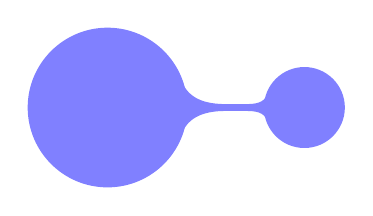
\begin{tikzpicture}[concept color=blue!50,blue!50,outer sep=0pt]
  \node (n1) at (0,0)   [circle,minimum size=2cm,fill,draw,thick] {};
  \node (n2) at (2.5,0) [circle,minimum size=1cm,fill,draw,thick] {};

  \path (n1) to[circle connection bar] (n2);
\end{tikzpicture}
\end{codeexample}
    %
    Note that it is not a good idea to have more than one |to| operation
    together with the option |circle connection bar| in a single |\path|. Use
    the |edge| operation, instead, for creating multiple connections and this
    operation creates a new scope for each edge.
\end{stylekey}

In a mindmap we sometimes want colors to change from one concept color to
another. Then, the connection bar should, ideally, consist of a smooth
transition between these two colors. Getting this right using shadings is a bit
tricky if you try this ``by hand'', so the  mindmap library provides a special
option for facilitating this procedure.

\begin{key}{/tikz/circle connection bar switch color=|from (|\meta{first color}|) to (|\meta{second color}|)|}
    This style works similarly to the |circle connection bar|. The only
    difference is that instead of filling the path with a single color a
    shading is used.
    %
\begin{codeexample}[]
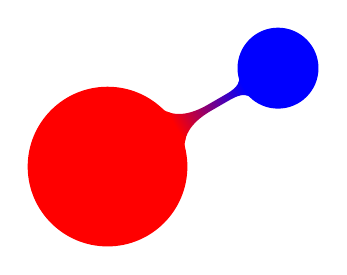
\begin{tikzpicture}[outer sep=0pt]
  \node (n1) at (0,0)    [circle,minimum size=2cm,fill,draw,thick,red] {};
  \node (n2) at (30:2.5) [circle,minimum size=1cm,fill,draw,thick,blue] {};

  \path (n1) to[circle connection bar switch color=from (red) to (blue)] (n2);
\end{tikzpicture}
\end{codeexample}
    %
\end{key}


\subsubsection{Tree Edges}

Most of the time, concepts in a mindmap are connected automatically when the
mindmap is built as a tree. The reason is that the |mindmap| installs a
|circle connection bar| path as the |edge from parent path|. Also, the
|mindmap| option takes care of things like setting the correct |draw| and
|outer sep| settings and some other stuff.

In detail, the |mindmap| option sets the |edge from parent path| to a path that
uses the to-path |circle connection bar| to connect the parent node and the
child node. The |concept color| option (locally) changes this by using
|circle connection bar switch color| instead with the from-color set to the old
(parent's) concept color and the to-color set to the new (child's) concept
color. This means that when you provide the |concept color| option to a |child|
command, the color will change from the parent's concept color to the specified
color.

Here is an example of a tree built in this way:
%
\begin{codeexample}[]
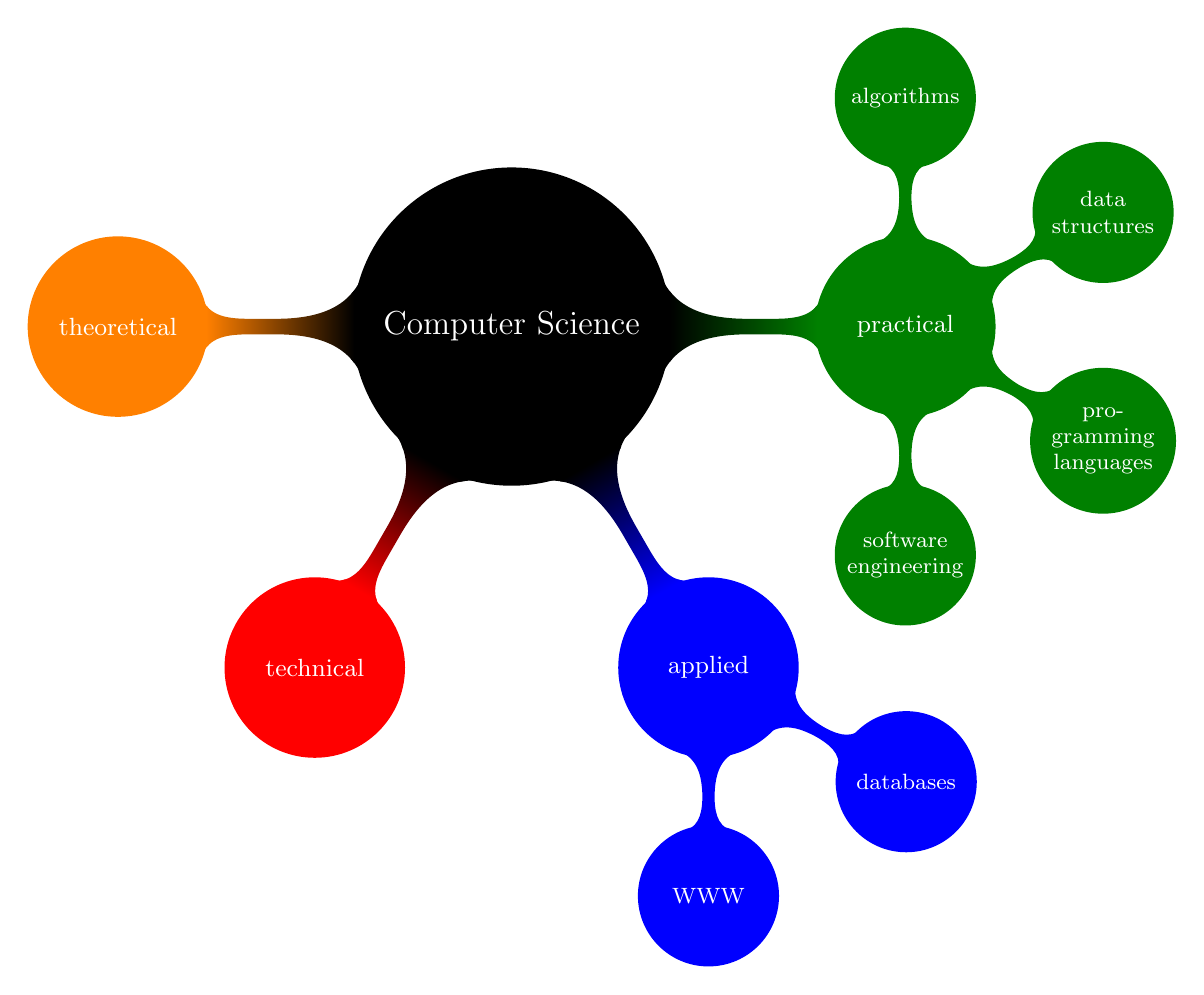
\begin{tikzpicture}
  \path[mindmap,concept color=black,text=white]
    node[concept] {Computer Science}
    [clockwise from=0]
    % note that `sibling angle' can only be defined in
    % `level 1 concept/.append style={}'
    child[concept color=green!50!black] {
      node[concept] {practical}
      [clockwise from=90]
      child { node[concept] {algorithms} }
      child { node[concept] {data structures} }
      child { node[concept] {pro\-gramming languages} }
      child { node[concept] {software engineer\-ing} }
    }
    child[concept color=blue] {
      node[concept] {applied}
      [clockwise from=-30]
      child { node[concept] {databases} }
      child { node[concept] {WWW} }
    }
    child[concept color=red] { node[concept] {technical} }
    child[concept color=orange] { node[concept] {theoretical} };
\end{tikzpicture}
\end{codeexample}


\subsection{Adding Annotations}

An \emph{annotation} is some text outside a mindmap that, unlike an extra
concept, simply explains something in the mindmap. The following style is
mainly intended to help readers of the code see that a node in an annotation
node.

\begin{stylekey}{/tikz/annotation}
    This style indicates that a node is an annotation node. It includes the
    style |every annotation|, which allows you to change this style in a
    convenient fashion.
    %
\begin{codeexample}[]
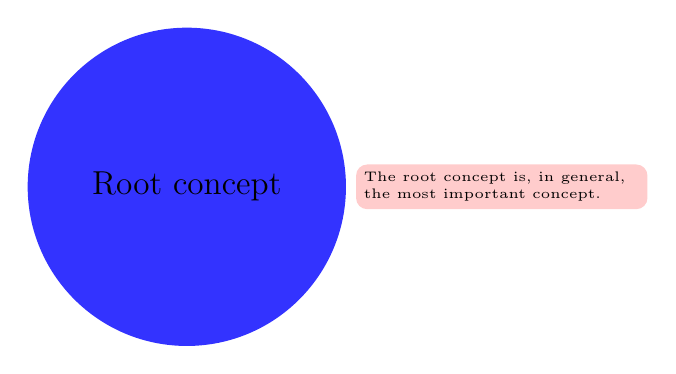
\begin{tikzpicture}
  [mindmap,concept color=blue!80,
  every annotation/.style={fill=red!20}]
  \node [concept] (root)  {Root concept};

  \node [annotation,right] at (root.east)
  {The root concept is, in general, the most important concept.};
\end{tikzpicture}
\end{codeexample}
    %
    \begin{stylekey}{/tikz/every annotation}
        This style is included by |annotation|.
    \end{stylekey}
\end{stylekey}


%%% Local Variables:
%%% mode: latex
%%% TeX-master: "pgfmanual-pdftex-version"
%%% End:
